\chapter{Evaluation}\label{chap:evaluation}


\section{Empirical Evaluation}
To prove that our technique is beneficial, we conduct a standard empirical evaluation on PO domains and compare the runtime of PO planners vs. transformation + TO planners

%\begin{tabular}{lcccccl}\toprule
%	& \multicolumn{3}{c}{$\tol=\tols$} & \multicolumn{3}{c}{$\tol=\told$}
%	\\\cmidrule(lr){2-4}\cmidrule(lr){5-7}
%	& $mv$  & Rel.~err & Time    & $mv$  & Rel.~err & Time\\\midrule
%	trigmv    & 11034 & 1.3e-7 & 3.9 & 15846 & 2.7e-11 & 5.6 \\
%	trigexpmv & 21952 & 1.3e-7 & 6.2 & 31516 & 2.7e-11 & 8.8 \\
%	trigblock & 15883 & 5.2e-8 & 7.1 & 32023 & 1.1e-11 & 1.4e1\\
%	expleja   & 11180 & 8.0e-9 & 4.3 & 17348 & 1.5e-11 & 6.6 \\\bottomrule
%\end{tabular}


% https://ojs.aaai.org/index.php/ICAPS/article/view/15959/15770
% HyperTension
% Pand Pro Pand SaT GBFS Add (th, s, th+s)


\subsection{Hardware Setup}
The following benchmark used ?GB RAM, %8GB RAM
Nectar cores, threads, processor, %Intel(R) Core(TM) i7-10510U CPU @ 1.80GHz  (Total Cores 4; Total Threads 8)
Nectar OS, and %Ubuntu 20.04.4 LTS
C++


Full Tables in Appendix. Plots/Tables of relevant properties, e.g.
\begin{center}
	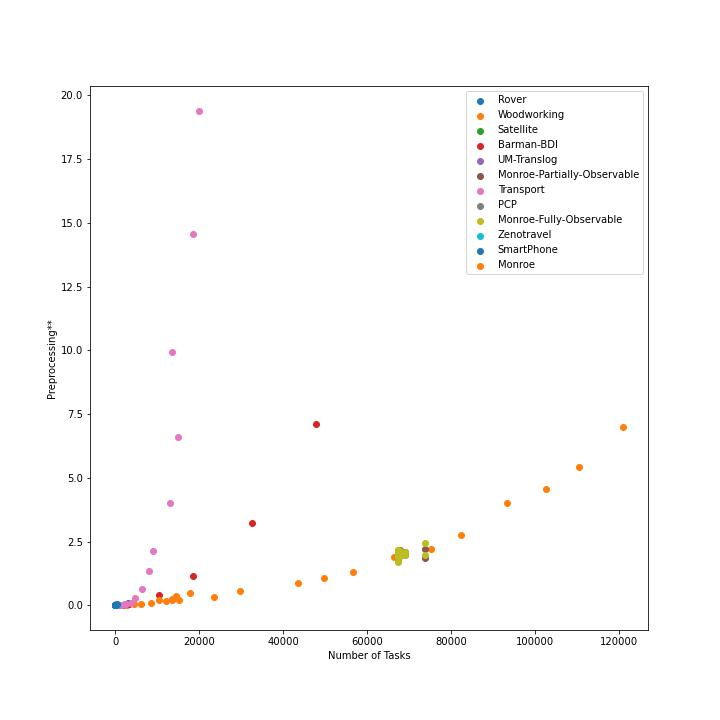
\includegraphics[scale=0.4]{../ipc2020-domains/Preprocessing**_vs_Tasksnotlog.jpg}
\end{center}

\begin{center}
	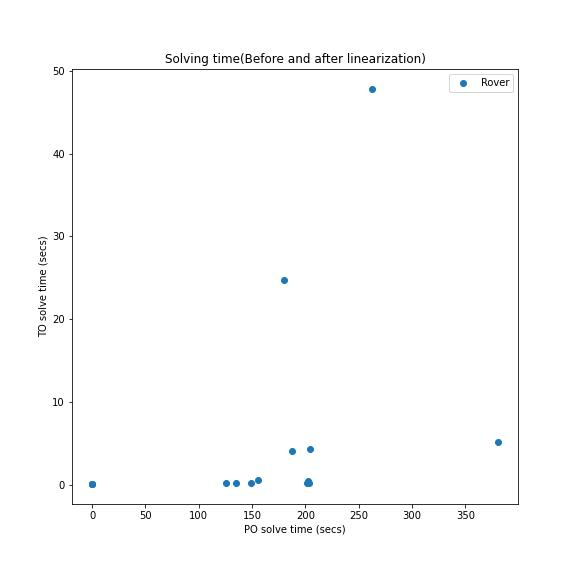
\includegraphics[scale=0.4]{../ipc2020-domains/Time_comparision.jpg}
\end{center}

\begin{enumerate}
	\item None of the instances can be linearized.
	\item Despite this, ?percent of linearized problems are solvable.
	\item The additional processing time is within the same order of time as the time needed for grounding and a tiny fraction of the overall time $\sim$
	\item We compare the ratio of (Grounding + Pre-processing time + TO solve time) to (Grounding + PO solve time), as those
	are the steps needed to solve the respective problems. The average solve time for the TO problem is ?? percent of the PO problem, for all problems.
	\item Difference in reduction of total solving time influenced most by ? (e.g. domain, recursiveness of problem, percentage of linearizable methods, etc)
\end{enumerate}